It is probable that your school has a variety of textbooks and old donated resource books hidden away in the headmasters office or in the Academic Office.  This books aren't being used because your school probably has no way of managing a system that will ensure books won't be stolen or damaged. \\

Conversely, you may be at a school that already has a library, but it is constantly locked or students never seem to use it.  Have no fear.  There are easy ways to overcome these challenges and get your students reading and using the materials your school already has available. \\
\begin{center}
\setlength\fboxsep{0pt}
\setlength\fboxrule{2pt}
\fbox{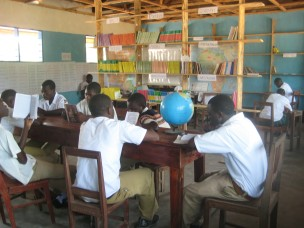
\includegraphics[scale=0.09]{IMG_3883.JPG}}
\end{center}

\section{Steps for Creating a Library}
\begin{enumerate}
\item Collect the books in your school, leaving one copy of each in the Academic office. Ask for book donations through organizations like Read International or Books for Africa.  Your District Education Officer should know about both of these NGOs as they are extremely active in Tanzania and usually consult the DEO before making donations. You will get some outdated material as well as some amazing donations. You could also have businesses donate bookshelves, tables and chairs in exchange for having a business name engraved right on the supplies donated.

\item Ask for monetary donations through your school, PPCP or SPA grants to build tables and shelves.

\item Organize your library once you have enough material. Figure out how you want it displayed and organized. Maybe you want to organize by subject or have a section that is textbooks and another that is reference.  You could also organize by form.  Make sure you get students involved at this stage.

\item Create a catalog system and inventory so you can keep track of which books are where in the library. Try writing the number of books in each subject on the shelf so you can quickly take daily inventory to see what is missing.

\item Take applications for student librarians. Usually one student per form is appropriate. Find students that are passionate about studying but can also stand up to noise makers. Too many can make things complicated.  Develop a set of rules together for the Library.  Can students check out books or are they only allowed to be used in the library? Should students be allowed to bring in bags? How many students can use the library at one time?

\item Develop a monitoring program.  The library can only be used when the teacher or a student librarian is present. Have students sign in and out when they come into the library.  Student librarians should count all the books at the end of each day.  If a book is missing, you know who used the library and when. This way the book can easily be recovered.

\item Encourage the students to use the library.  Schedule library time into the school time table when there is an open period.  Encourage teachers to use it.  Hold class there rahter than bring books to class. Hang up students work in the library. Have movie nights there for students who live on or near campus. Try to develop a culture of reading.

\item Look for ways to improve your library.  Be sure to always include Tanzanian staff to create sustainability. 

\end{enumerate}